\documentclass[12pt]{article}
\usepackage[utf8]{inputenc}
\usepackage[T2A]{fontenc}
\usepackage[english, russian]{babel}
\usepackage[a4paper, includefoot, left=1.5cm, right=1cm, top=1cm, bottom=1.5cm, headsep=1cm, footskip=1cm]{geometry}
\usepackage{makecell}
\usepackage{amsmath}
\usepackage{graphicx}
\usepackage{enumitem}
\usepackage{svg}
\usepackage{multirow}
\usepackage{hyperref}
%\newcolumntype{C}{>{$}c<{$}}

\newcounter{point}
\newenvironment{point}[1]{
    \refstepcounter{point}
    \vspace{2mm}
    \textbf{\emph{\thepoint. #1}}
    \vspace{1mm}
}
{
    
}


\newcommand{\makeheader}{
\noindent
    \begin{minipage}[t]{0.2\textwidth}
        \vspace{0mm}
        
\includegraphics[width=\textwidth]{images/au-logo-shadow.eps}
    \end{minipage}
    \hfill
    \begin{minipage}[t]{0.75\textwidth}
        \footnotesize ФЕДРЕРАЛЬНОЕ ГОСУДАРСТВЕННОЕ БЮДЖЕТНОЕ УЧРЕЖДЕНИЕ \\ ВЫСШЕГО ОБРАЗОВАНИЯ И НАУКИ
        \normalsize \\
        \textbf{САНКТ-ПЕТЕРБУРГСКИЙ НАЦИОНАЛЬНЫЙ \\ ИССЛЕДОВАТЕЛЬСКИЙ АКАДЕМИЧЕСКИЙ \\ УНИВЕРСИТЕТ ИМЕНИ Ж. И. АЛФЁРОВА \\ РОССИЙСКОЙ АКАДЕМИИ НАУК \qquad \qquad \qquad \qquad \quad \quad \ \ \(  \)}
        \vspace{0mm}
    \end{minipage}
    \noindent \rule{185mm}{1pt}
    \vspace{5mm}

    \large
    \noindent Группа \underline{201.1} \noindent\rule{52mm}{0.4pt} \hspace{25mm} К работе допущен \noindent\rule{34mm}{0.4pt} \\ %\noindent\rule{60mm}{0.4pt}
     Студент \underline{Кононов А, Ясинский М} \noindent\rule{0mm}{0.4pt} \hspace{32mm} Работа выполнена \noindent\rule{34mm}{0.4pt}\\ % \noindent\rule{58mm}{0.4pt}
     Преподаватель \underline{Василькова Е. И.} \hspace{34mm} Отчет принят \noindent\rule{43mm}{0.4pt}
     Лаборант \noindent\rule{55mm}{0.4pt} \\
    \vspace{5mm}
}

\newcommand{\makelabheading}[2]{
    \begin{center}
        \LARGE \textbf{Рабочий протокол и отчет по \\ лабораторной работе №#1}
    \end{center}
    \vspace{-3mm}
    \begin{center}
        \Large #2
    \end{center}
    \vspace{-8mm}
    \noindent \rule{185 mm}{1pt}
    \vspace{5mm}
}
\newcounter{tablenumber}
\newcommand{\gimmeheading}[1]{
    \refstepcounter{tablenumber}
    \begin{center}
        \underline{Таблица \thetablenumber}: #1
    \end{center}
}

\newcommand{\devices}{
    \begin{center}
        \begin{tabular}{ |c|c|c|c|c| }
            \hline
            № & Наименование & Тип прибора & \makecell{Исследуемый \\ диапазон} & \makecell{Погрешность \\ прибора} \\
            \hline
            1 & Тесламетр    & Электронный  & \(0 \div 1100\) мТл & 1 мТл  \\
            \hline
            2 & Вольтметр    & Электронный  & \(0 \div 10\) мкВ & 0,1 мкВ  \\
            \hline
            3 & Амперметр    & Электронный  & \(0 \div 5\) А & 0,1 А  \\
            \hline
        \end{tabular}
    \end{center}
    \gimmeheading{перечень измерительных приборов}
}
\newcommand{\izmerenia}{
    \begin{center}
\begin{tabular}{|r|r|r|}
\hline
\multicolumn{1}{|l|}{№} & \multicolumn{1}{l|}{$B$, мТл} & \multicolumn{1}{l|}{$U_{\perp}$, мкВ} \\ \hline
1                       & 56                          & 0,9                             \\ \hline
2                       & 155                         & 1,1                             \\ \hline
3                       & 257                         & 1,7                             \\ \hline
4                       & 356                         & 2,3                             \\ \hline
5                       & 456                         & 2,7                             \\ \hline
6                       & 555                         & 3,4                             \\ \hline
7                       & 656                         & 3,9                             \\ \hline
8                       & 756                         & 4,4                             \\ \hline
9                       & 856                         & 4,7                             \\ \hline
10                      & 956                         & 5,1                             \\ \hline
11                      & 1055                        & 5,6                             \\ \hline
\end{tabular}
    \end{center}
    \gimmeheading{результаты измерений}
}
\newcommand{\vichislenia}{
    \begin{center}
\begin{tabular}{|l|r|r|r|r|}
\hline
№  & \multicolumn{1}{l|}{$1000/T$, $\text{К}^{-1} \cdot 1000$} & \multicolumn{1}{l|}{$G \cdot 1000$, $\text{Ом}^{-1} \cdot 1000$} & \multicolumn{1}{l|}{$\sigma$, $(\text{Ом} \cdot \text{м})^{-1}$} & \multicolumn{1}{l|}{$\ln(\sigma)$} \\ \hline
1  & 2,392                                                                            & 76,046                                                                                                                         & 38,02                                                                                                                                            & 3,64                                           \\ \hline
2  & 2,451                                                                            & 59,524                                                                                                                         & 29,76                                                                                                                                            & 3,39                                           \\ \hline
3  & 2,513                                                                            & 44,643                                                                                                                         & 22,32                                                                                                                                            & 3,11                                           \\ \hline
4  & 2,577                                                                            & 33,411                                                                                                                         & 16,71                                                                                                                                            & 2,82                                           \\ \hline
5  & 2,646                                                                            & 25,870                                                                                                                         & 12,93                                                                                                                                            & 2,56                                           \\ \hline
6  & 2,681                                                                            & 22,818                                                                                                                         & 11,41                                                                                                                                            & 2,43                                           \\ \hline
7  & 2,717                                                                            & 20,833                                                                                                                         & 10,42                                                                                                                                            & 2,34                                           \\ \hline
8  & 2,755                                                                            & 18,999                                                                                                                         & 9,50                                                                                                                                             & 2,25                                           \\ \hline
9  & 2,793                                                                            & 17,857                                                                                                                         & 8,93                                                                                                                                             & 2,19                                           \\ \hline
10 & 2,833                                                                            & 16,878                                                                                                                         & 8,44                                                                                                                                             & 2,13                                           \\ \hline
11 & 2,874                                                                            & 16,529                                                                                                                         & 8,26                                                                                                                                             & 2,11                                           \\ \hline
12 & 2,915                                                                            & 16,393                                                                                                                         & 8,20                                                                                                                                             & 2,10                                           \\ \hline
13 & 2,959                                                                            & 16,393                                                                                                                         & 8,20                                                                                                                                             & 2,10                                           \\ \hline
14 & 3,003                                                                            & 16,529                                                                                                                         & 8,26                                                                                                                                             & 2,11                                           \\ \hline
15 & 3,049                                                                            & 16,807                                                                                                                         & 8,40                                                                                                                                             & 2,13                                           \\ \hline
16 & 3,096                                                                            & 17,241                                                                                                                         & 8,62                                                                                                                                             & 2,15                                           \\ \hline
17 & 3,145                                                                            & 17,699                                                                                                                         & 8,85                                                                                                                                             & 2,18                                           \\ \hline
18 & 3,195                                                                            & 18,349                                                                                                                         & 9,17                                                                                                                                             & 2,22                                           \\ \hline
19 & 3,247                                                                            & 18,868                                                                                                                         & 9,43                                                                                                                                             & 2,24                                           \\ \hline
20 & 3,300                                                                            & 19,608                                                                                                                         & 9,80                                                                                                                                             & 2,28                                           \\ \hline
\end{tabular}
\end{center}
\gimmeheading{вычесление удельной проводимости и ее логарифма}
}
\newcommand{\pogrehnosti}{
    \begin{center}
    \begin{tabular}{|l|r|r|r|r|r|}
\hline
№  & \multicolumn{1}{l|}{$\Delta r_{0}$, м $\cdot 10^{-7}$} & \multicolumn{1}{l|}{$\Delta q_{0}$, Кл $\cdot 10^{-19}$} & \multicolumn{1}{l|}{$\Delta r$, м $\cdot 10^{-7}$} & \multicolumn{1}{l|}{$\Delta q$, Кл $\cdot 10^{-19}$} & \multicolumn{1}{l|}{$\Delta e$, Кл $\cdot 10^{-19}$} \\ \hline
1  & 0,003                                                & 0,28                                                   & 0,003                                               & 0,27                                                  & 0,13                                                  \\ \hline
2  & 0,001                                                & 0,43                                                   & 0,001                                               & 0,42                                                  & 0,14                                                  \\ \hline
3  & 0,002                                                & 0,81                                                   & 0,002                                               & 0,79                                                  & 0,15                                                  \\ \hline
4  & 0,001                                                & 0,15                                                   & 0,001                                               & 0,14                                                  & 0,14                                                  \\ \hline
5  & 0,003                                                & 0,69                                                   & 0,003                                               & 0,68                                                  & 0,17                                                  \\ \hline
6  & 0,002                                                & 0,20                                                   & 0,002                                               & 0,20                                                  & 0,20                                                  \\ \hline
7  & 0,007                                                & 2,02                                                   & 0,007                                               & 2,01                                                  & 0,18                                                  \\ \hline
8  & 0,007                                                & 0,35                                                   & 0,007                                               & 0,34                                                  & 0,34                                                  \\ \hline
9  & 0,005                                                & 2,13                                                   & 0,005                                               & 2,11                                                  & 0,15                                                  \\ \hline
10 & 0,006                                                & 2,73                                                   & 0,006                                               & 2,71                                                  & 0,15                                                  \\ \hline
11 & 0,003                                                & 0,27                                                   & 0,003                                               & 0,27                                                  & 0,13                                                  \\ \hline
12 & 0,002                                                & 0,17                                                   & 0,002                                               & 0,16                                                  & 0,16                                                  \\ \hline
\end{tabular}

    \end{center}
    \gimmeheading{погрешности измерений}
}

\begin{document}
    \makeheader
    \makelabheading{4}{Эффект Холла в проводнике}

    \begin{point}{Цель работы}
        \par Изучить эффект Холла в проводнике
    \end{point}

    \begin{point}{Задачи, решаемые при выполнении работы}
        \par -Измерение зависимости холловской электродвижущей силы от индукции магнитного поля
        \par -Определение концентрации образца и подвижности основных носителей заряда
        \par -Определение значения константы Холла
    \end{point}

    \begin{point}{Объект исследования}
        \par Эффект Холла при взаимодействии проводника с электромагнитным полем.
    \end{point}

    \begin{point}{Метод экспериментального исследования}
        \par Измерение зависимости поперечного напряжения от величины индукции магнитного поля.
    \end{point}

    \begin{point}{Рабочие формулы и исходные данные}
        \begin{itemize}
            \item Константа холла
            \begin{equation}
                R = \frac{U_{\perp}d}{IB}
            \end{equation}
            где $R$ - константа Холла
            \par $U_{\perp}$ - поперечное напряжение
            \par $d$ - ширина проводника
            \par $I$ - сила тока
            \par $B$ - индукция магнитного поля

            \item Концентрация носителей заряда
            \begin{equation}
                n = \frac{1}{eR}
            \end{equation}
            где $e$ - заряд электрона

            \item Подвижность носителей заряда
            \begin{equation}
                \mu = \frac{R}{\rho}
            \end{equation}
            где $\rho$ - удельная проводимость образца металла
%            \item Среднеквадратичное отклонение (СКО)
%            \begin{equation}
%                \sigma_{\text{t}} = \sqrt{\frac{1}{N}\cdot\sum\limits_{i = 1}^N(t_{\text{i}} - \overline{t})^2}
%            \end{equation}
%            где $N$ - размер выборки
%            \item СКО среднего значения
%            \begin{equation}
%                \sigma_{\overline{\text{t}}} = \frac{\sigma_{\text{t}}}{\sqrt{N - 1}}
%            \end{equation}
%            \item Случайная погрешность
%            \begin{equation}
%                \Delta t_{\text{сл}} = t_{\alpha N}\sigma_{\overline{\text{t}}}
%            \end{equation}
%            где $t_{\alpha N}$ - коэффициент Стьюдента для данного значения доверительной вероятности $t$. В нашем случае для
%            $\alpha = 0,9$ и $N = 12$: $t_{\alpha N} = 1,80$
%%            \item Полная абсолютная погрешность измерения
%            \begin{equation}
%                \Delta t = \sqrt{(\Delta t_{\text{пр}})^2 + (\Delta t_{\text{сл}})^2}
%            \end{equation}
%            где $\Delta t_{\text{пр}}$ - приборная погрешность
        \end{itemize}
    \end{point}

    \begin{point}{Измерительные приборы}
        \devices
    \end{point}

    \begin{point}{Схема установки}
        \par
        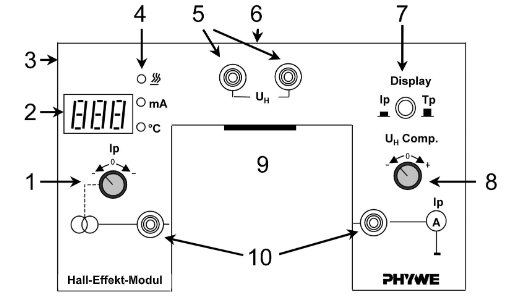
\includegraphics[width=\textwidth]{images/scheme.png}
        \begin{center}
        \underline{Рисунок 1}: Ручка регулирования тока через образец $I_{P}$ (1);
            Цифровой индикатор, показывающий, ток через образец (2);
            Резьбовое отверстие для крепления модуля (3);
           Светодиодные индикаторы, показывающие включение режима
нагрева образца, а также режим индикации либо тока через образец, либо температуры образца (4);
           Клеммы для измерения поперечного напряжения на образце $U_{\perp}$ (5);
          Отверстие для крепления магнитного зонда  (6);
           нопка выбора режима индикации: если кнопка нажата, то измеряется ток через образец $I_{P}$, если отжата – то температура образца $T_{P}$ (7);
          Ручка компенсации поперечного напряжения (8);
          Выемка для крепления сменной платы с электрическим разъёмом  (9);
         Клеммы для измерения продольного напряжения на образце $U_{P}$ (10).
        \end{center}
    \end{point}

    \begin{point}{Результаты прямых измерений и их обработки (таблицы, примеры расчетов)}
        \izmerenia
    \end{point}

    \begin{point}{Расчет результатов косвенных измерений (таблицы, примеры расчетов)}
        \par Установив постоянный ток $I = 2,5 \text{А}$ через образец, и, снимая поперечное напряжение на нем в процессе эксперимента,
        а так же зная размеры образца $d = 25 \text{мкм}$, мы можем посчитать константу Холла изучаемого металла (цинка):
        \[R = \frac{\Delta U_{\perp}d}{\Delta B I}\]
        \par
        Найдем отношение изменения поперечного напряжения к изменению магнитной индукции из аппроксимации, методом наименьших квадратов
        \par
        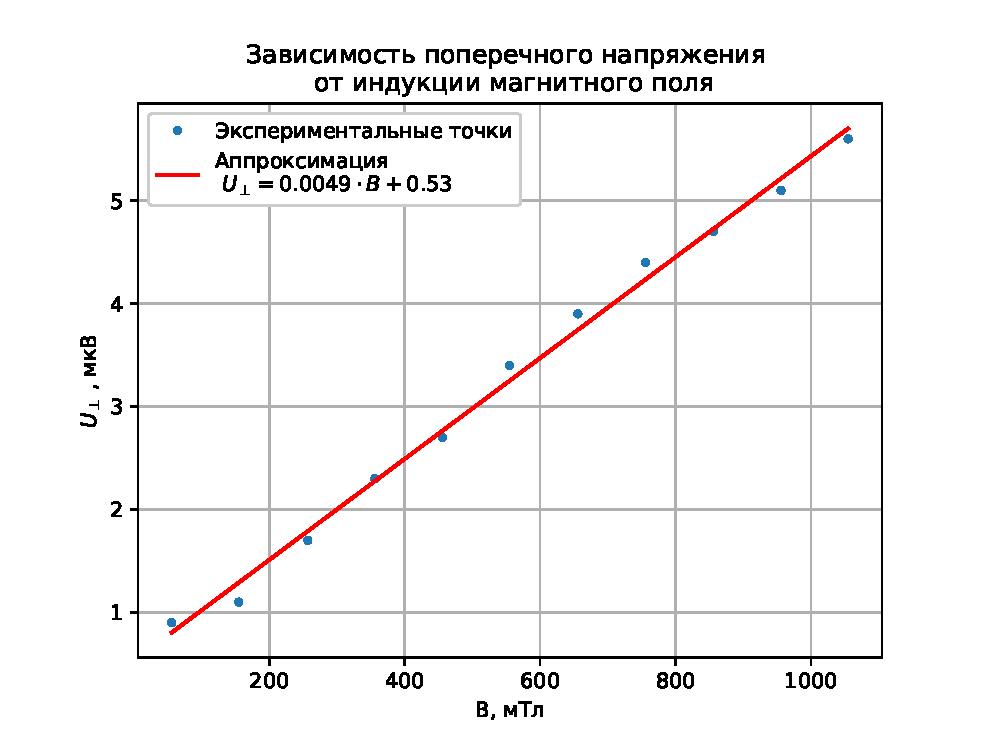
\includegraphics[width=\textwidth]{images/holl.eps}
        \begin{center}
        \underline{График 1}: Зависимость поперечного напряжения от магнитной индукции
        \end{center}
        \par
        С помощью МНК и ковариационной матрицы получили следующую зависимость:
        \[ U_{\perp} = 0,0049 \cdot B + 0,53\]
        \par
        где
        \[\frac{\Delta U_{\perp}}{\Delta B} = 0,0049 \pm 0,0001 \frac{\text{мкВ}}{\text{мТл}}\]
        \par таким образом константа Холла для нашего образца равна:
        \[R = (4,9 \pm 0,1) \cdot 10^{-11} \frac{\text{В} \cdot \text{м}}{\text{Тл} \cdot \text{А}} \]
        \par Зная заряд электрона $e = 1,6 \cdot 10^{-19} \text{Кл}$, найдем концентрацию носителей заряда:
        \[n = (12,8 \pm 0,3) \cdot 10^{28} \text{ м}^{-3} \]
        \par А так же, зная удельное сопротивления для цинка $\rho = 5,4 \cdot 10^{-8} \text{ Ом} \cdot \text{м}$, найдем подвижность зарядов в нем:
        \[\mu = (0,90 \pm 0,02) \cdot 10^{-3} \frac{\text{м}^2}{\text{В} \cdot \text{с}} \]
        %\vichislenia
    \end{point}

%    \begin{point}{Расчет погрешностей измерений (для прямых и косвенных измерений)}
%        \par Всвязи с однократностью проводимых опытов будем считать погрешность прямых измерений равной приборной погрешности
%        \par Найдем погрешности радиуса капли. Начнем с частных производных:
%        \par $B = \sqrt{4,5 \frac{\eta}{\left( \rho_{2} - \rho_{1} \right)g}}$ - Константа
%        \[
%            \frac{\partial r_{0}}{\partial l_{2}} = \frac{B}{2\sqrt{l_{2}t_{2}}}
%        \]
%        \[
%            \frac{\partial r_{0}}{\partial t_{2}} = -\frac{B}{2t_{2}}\sqrt{\frac{l_{2}}{t_{2}}}
%        \]
%        \[\Downarrow \]
%        \[\Delta r_{0} = B \sqrt{\left(\frac{\Delta l_{2}}{2\sqrt{l_{2}t_{2}}} \right)^2 + \left( \frac{\Delta t_{2}}{2t_{2}}\sqrt{\frac{l_{2}}{t_{2}}} \right)^2}\]
%        \par
%        \par Теперь найдем погрешность зарядка капли:
%        \par $C = 6 \pi \eta$ - Константа
%        \par $\Delta d = 0,1 \cdot 10^{-3} \text{ м}$ - погрешность расстояния между пластинами
%        \[
%            \frac{\partial q_{0}}{\partial l_{1}} = \frac{C d r_{0}}{U t_{1}}
%        \]
%        \[
%            \frac{\partial q_{0}}{\partial l_{2}} = \frac{C d r_{0}}{U t_{2}}
%        \]
%        \[
%            \frac{\partial q_{0}}{\partial t_{1}} = -\frac{C d l_{1} r_{0}}{U t_{1}^2}
%        \]
%        \[
%            \frac{\partial q_{0}}{\partial t_{2}} = -\frac{C d l_{2} r_{0}}{U t_{2}^2}
%        \]
%        \[
%            \frac{\partial q_{0}}{\partial r_{0}} = \frac{C d}{U} \left( \frac{l_{1}}{t_{1}} + \frac{l_{2}}{t_{2}} \right)
%        \]
%        \[
%            \frac{\partial q_{0}}{\partial d} = \frac{C r_{0}}{U} \left( \frac{l_{1}}{t_{1}} + \frac{l_{2}}{t_{2}} \right)
%        \]
%        \[
%            \frac{\partial q_{0}}{\partial U} = -\frac{C d r_{0}}{U^2} \left( \frac{l_{1}}{t_{1}} + \frac{l_{2}}{t_{2}} \right)
%        \]
%        \[\Downarrow \]
%        \[\Delta q_{0} = \sqrt{\left( \frac{\partial q_{0}}{\partial l_{1}} \Delta l_{1} \right)^2 + \left( \frac{\partial q_{0}}{\partial l_{2}} \Delta l_{2}  \right)^2 + \left( \frac{\partial q_{0}}{\partial t_{1}} \Delta t_{1}  \right)^2 + \left( \frac{\partial q_{0}}{\partial t_{2}} \Delta t_{2}  \right)^2 + \left( \frac{\partial q_{0}}{\partial r_{0}} \Delta r_{0}  \right)^2 + }\]
%        \[ \overline{ + \left( \frac{\partial q_{0}}{\partial d} \Delta d  \right)^2 + \left( \frac{\partial q_{0}}{\partial U} \Delta U  \right)^2}\]
%    \par Погрешность для уточненного радиуса
%        \[\Delta r = \frac{r_{0} \Delta r_{0}}{\sqrt{r_{0}^2 + 0,25 A^2}}\]
%    \par Погрешность уточненного заряда капли
%        \[
%            \frac{\partial q}{\partial q_{0}} = \left( 1 + \frac{A}{r} \right) ^ {-1,5}
%        \]
%        \[
%            \frac{\partial q}{\partial r} = \frac{1,5 A q_{0}}{r^2 \left( 1 + \frac{A}{r} \right) ^ {2,5}}
%        \]
%        \[\Downarrow \]
%        \[\Delta q = \sqrt{\left( \frac{\partial q}{\partial q_{0}} \Delta q_{0} \right)^2 + \left( \frac{\partial q}{\partial r} \Delta r \right)^2}\]
%    \par Погрешность элементарного заряда
%        \[\Delta e_{i} = \frac{\Delta q_{i}}{n_{i}}\]
%    \par Результаты погрешностей приведены в таблице
    %    \[
    %        \frac{\partial I_1}{\partial h_{\text{01}}} = -\frac{5,156^2 \cdot (49,287 \cdot 9,81 \cdot 6,5 \cdot 10^{-5} - 0,0093)}{2|(6,0 - 46,5) \cdot 10^{-2}|^2} = -0,02
    %    \]
    %    \[
    %        \frac{\partial I_1}{\partial M_{\text{t}}} = -\frac{6,5 \cdot 10^{-2} \cdot 5,156^2}{2|(6,0 - 46,5) \cdot 10^{-2}|} = -2,2
    %    \]
    %    \[
    %        \frac{\partial I_1}{\partial t} = -\frac{6,5 \cdot 10^{-2} \cdot 5,156(49,287 \cdot 9,81 \cdot 6,5 \cdot 10^{-5} - 0,0093)}{|(6,0 - 46,5) \cdot 10^{-2}|} = -0,002
    %    \]
    %    \[\Downarrow \]
    %    \[\Delta I_1 = \sqrt{\left( 1,4 \cdot 0,00034\right)^2 + \left(2,1 \cdot 0,001\right)^2 + \left(-0,02 \cdot 0,001\right)^2 + \left(-2,2 \cdot 0,0002 \right)^2}\]
    %    \[\overline{+ \left(-0,002 \cdot 0,001 \right)^2} = 0,002 \text{ кг} \cdot \text{м}^2 \]
    %\par Аналогично остальные эксперименты. Результаты погрешностей предоставлены в таблице.
    %\par
%    \pogrehnosti
%    \end{point}

%    \begin{point}{Окончательные результаты}
%        \par Усредняя значение элементарного заряда и его погрешности получаем:
%        \[ e = 1,67 \cdot 10^{-19} \text{Кл; } \Delta e_{\text{приб}} = 0,17 \cdot 10^{-19} \text{Кл}\]
%        \par Считая все погрешности элементарного заряда случайными величинами, рассчитали истинную погрешность через СКО
%        \[\sigma_{\Delta e} = 0,213 \cdot 10^{-19}\]
%        \[\sigma_{\overline{\Delta e}} = 0,064 \cdot 10^{-19}\]
%        \[\Delta e_{\text{случ}} = 0,11 \cdot 10^{-19} \text{Кл}\]
%        \[\Delta e = 0,21 \cdot 10^{-19} \text{Кл}\]
%        \par Окончательный результат
%        \[e \pm \Delta e = \left( 1,67 \pm 0,21  \right) \cdot 10^{-19} \text{ Кл} \]
%        \par Построили график зависимости логарифма удельной проводимости от обратной температуры.
%        Найдем аппроксимацию левой части графика для вычисления собственной проводимости $Ge_{p+}$  и нахождения ширины запрещенной зоны $E_{g}$.
%        С помощью МНК получили следующую зависимость:
%        \[ ln(\sigma) = -4219 \cdot (1/T) + 13.72\]
%        Где $tg(\phi) = 4219 \text{ К}$.
%        Используя значения ковариационный матрицы МНК, можно найти погрешность $\Delta(tg(\phi)) = 91 \text{ К}$.
%        Зная постоянную Больцмана:
%        \newline $k = 8.617 \cdot 10^{-5} \text{ эВ/К}$, найдем ширину запрещенной зоны:
%        \[E_{g} = 2 \cdot 8.617 \cdot 10^{-5} \text{ эВ/К} \cdot 4219 \text{ К} = 0.727 \text{ эВ} \]
%        \[ \Delta(E_{g}) = 2k \cdot \Delta(tg(\phi)) = 0.016 \text{ эВ} \]
%        \par Окончательный результат:
%        \[ E_{g} = 0.727 \pm 0.016 \text{ эВ}\]
%        \par
%        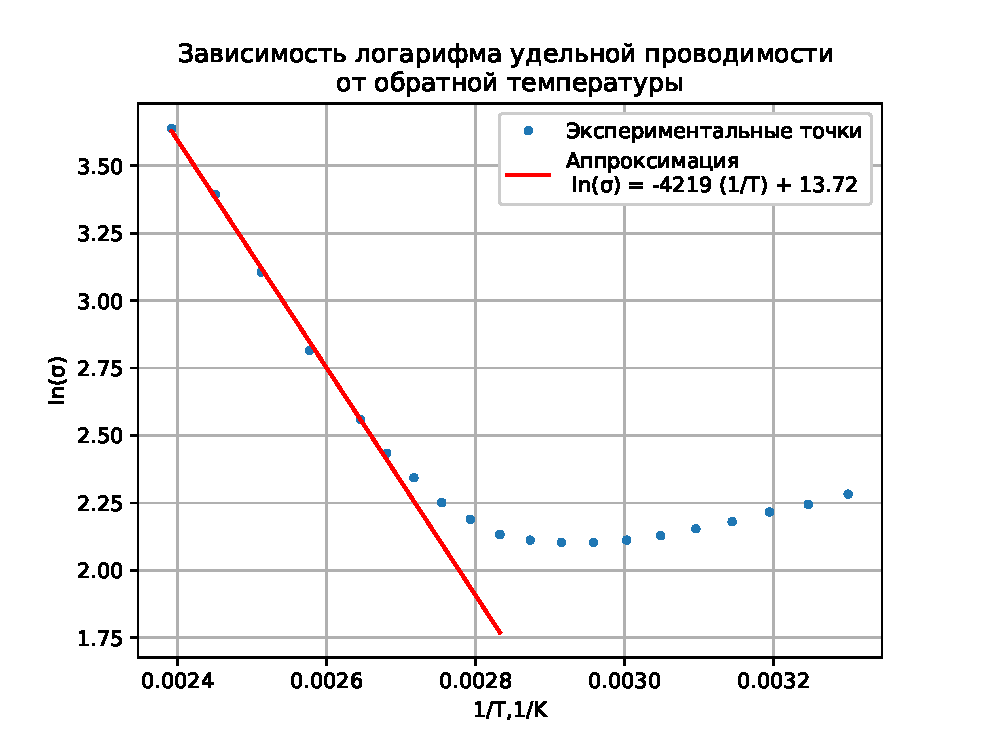
\includegraphics[width=\textwidth]{images/sigma.eps}
%        \begin{center}
%        \underline{График 1}: Зависимость логарифма удельной проводимости от обратной температуры        \end{center}
%        \par
%        \end{point}

    \begin{point}{Выводы и анализ результатов}
        \par В данной лабораторной работе нами была найдена константа Холла для цинка. Снимая зависимость поперечного напряжения от индукции магнитного поля, нами была расчитана константа Холла.
        В разных справочниках мы нашли разные табличные значения для этой константы. Самое близкое к нашему значению оказалось следующее:
        \[R^{\text{таблич}} = 4,0 \cdot 10^{-11} \frac{\text{м}^3}{\text{Кл}}\]
        \par В пределах погрешности найденная нами константа не совпадает с табличной, но по порядку они совпадают:
        \[|R^{\text{таблич}} - R| > \Delta R\]
        \[ R \sim R^{\text{таблич}} \sim 10^{-11} \frac{\text{м}^3}{\text{Кл}} \]
        \par Это может быть связанно с различными эффектами, например, температурой, от которой зависит константа Холла, а так же наличием примесей в нашем образце, которые могут влиять на различные электрические св-ва, в том числе и константу Холла.
        \par Еще нами была рассчитана концентрация и подвижность носителей заряда в Цинке.
        При этом рассчитанное значение концентрации согласуется с табличным в пределах погрешности:
        \[ n^{\text{таблич}} = 13,1 \cdot 10^{28} \text{ м}^{-3}\]
        \[ |n^{\text{таблич}} - n| \leq \Delta n \]
        \par А табличное значение подвижности для носителей заряда в цинке нам найти не удалось.
        \par Стоит отметить, что положительность константы Холла можно объяснить следующим образом: с увеличением индукции магнитного должна возрастать сила Лоренца, а значит и поперечное напряжение. Значит зависимость должна иметь положительный знак. Так как сила Лоренца, ток и магнитная индукция образуют правую тройку векторов, можем говорить о положительности поперечного напряжения.
        Если бы при тех же направлениях тока и магнитного поля, напряжение имело бы другой знак, это бы означало, что носители заряда имеют другой знак и поэтому сила лоренца направлена в другую сторону, образуя левую тройку векторов.
        Исходя из полученных результатов можем считать работу успешно выполненной.
    \end{point}
\end{document}
